\documentclass[12pt,en,a4paper]{article}
\usepackage{vntex}
\usepackage{enumerate}
\usepackage{array}
\usepackage{enumitem}
\usepackage{hyperref}
\usepackage{graphicx}
\usepackage{caption}
\usepackage{pgfplots}
\usepackage{amssymb}
\usepackage[open,openlevel=1]{bookmark}
\usepackage{comment}

\begin{document}
	\begin{table}[]
		\centering
		\begin{tabular}{|p{0.1\textwidth}|p{0.5\textwidth}|p{0.2\textwidth}|p{0.2\textwidth}|}
			\hline
			\multicolumn{4}{|c|}{GROUP --- MEMBER LIST} \\
			\hline
			No. & Name & ID & Role \\
			\hline
			1 & Nguyễn Hoàng & 1952255 & Blank \\
			\hline
			2 & Blank & Blank & Blank \\
			\hline
		\end{tabular}
	\end{table}
\pdfbookmark[0]{Problem 1}{prob1}
	\section*{Problem 1:}
	\begin{figure}[h]
		\begin{minipage}{0.5\textwidth}
			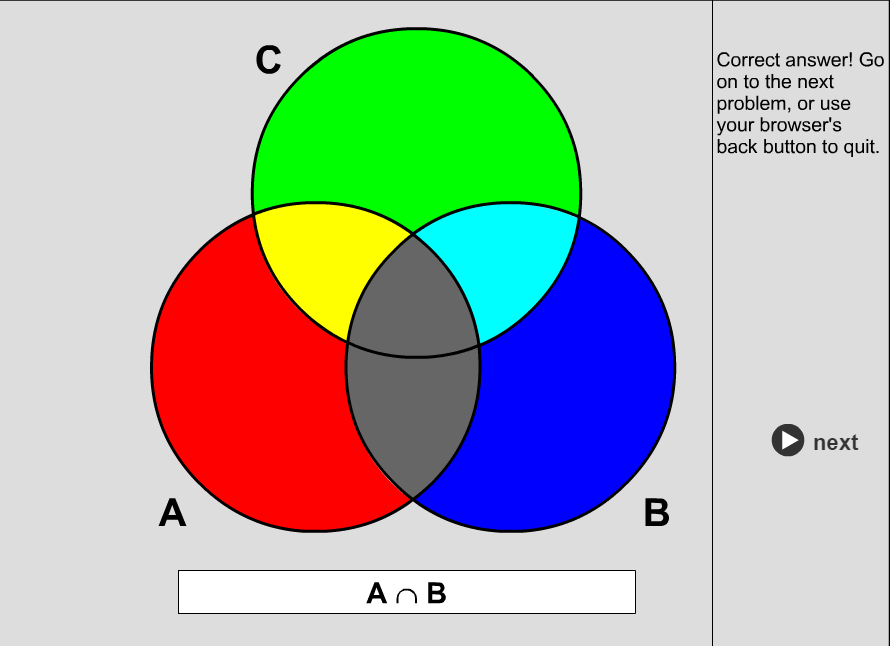
\includegraphics[width=1.0\textwidth]{SOL_set_1_1.png}
			\caption*{$A \cap B$}
			\label{fig:prob_1_1}
		\end{minipage}
		\begin{minipage}{0.5\textwidth}
			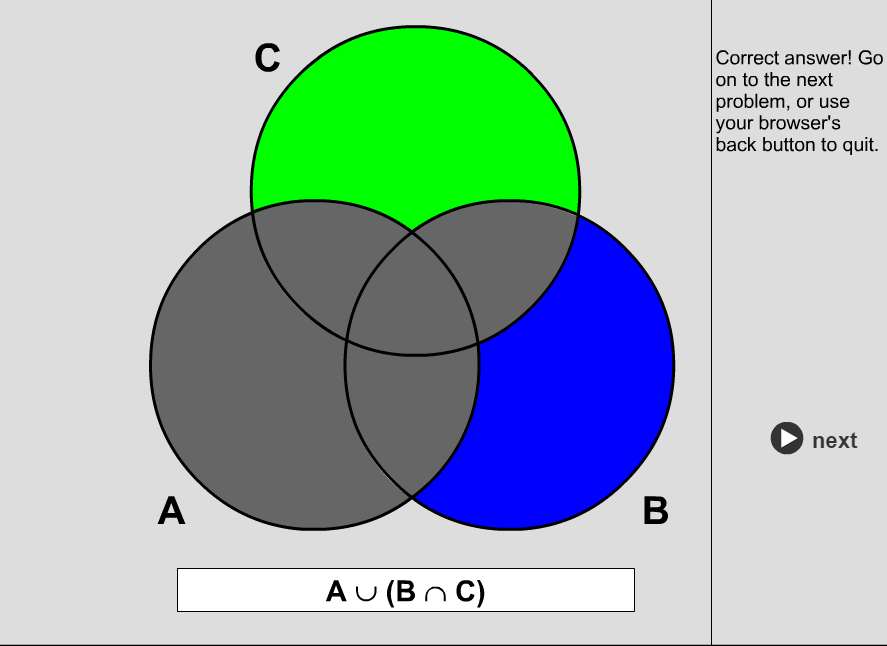
\includegraphics[width=1.0\textwidth]{SOL_set_1_2.png}
			\caption*{$A \cup (B \cap C)$}
			\label{fig:prob_1_2}
		\end{minipage}
	\end{figure}
	\begin{figure}[ht]
		\begin{minipage}{0.5\textwidth}
			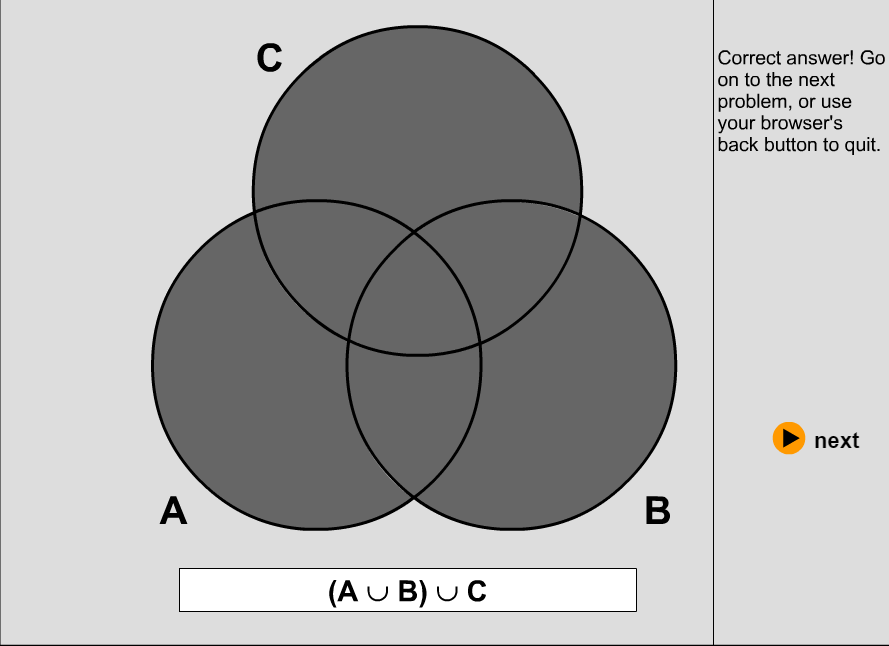
\includegraphics[width=1.0\textwidth]{SOL_set_1_3.png}
			\caption*{$(A \cup B) \cup C$}
			\label{fig:prob_1_3}
		\end{minipage}
		\begin{minipage}{0.5\textwidth}
			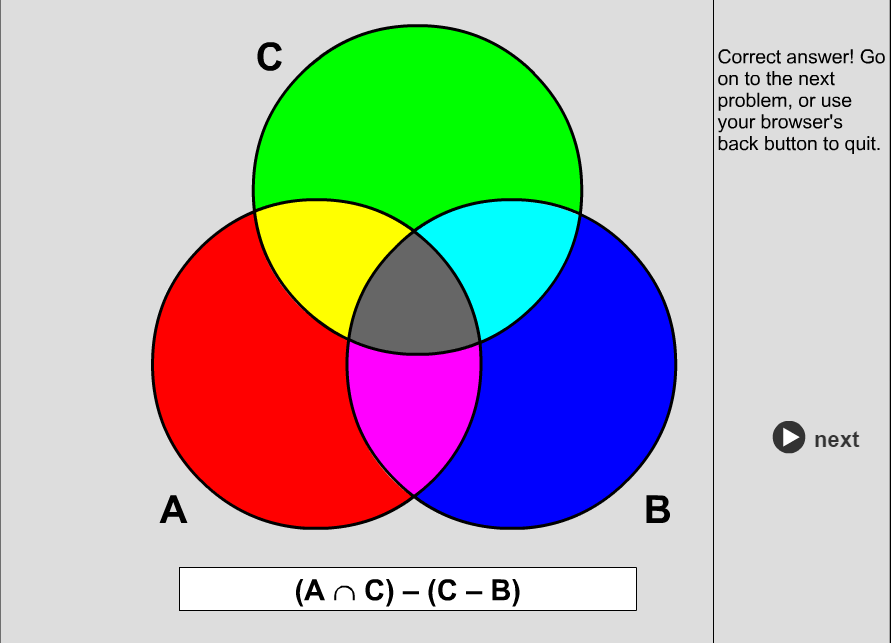
\includegraphics[width=1.0\textwidth]{SOL_set_1_4.png}
			\caption*{$(A \cap C)-(C-B)$}
			\label{fig:prob_1_4}
		\end{minipage}
	\end{figure}
	\begin{figure}[ht]
		\begin{minipage}{0.5\textwidth}
			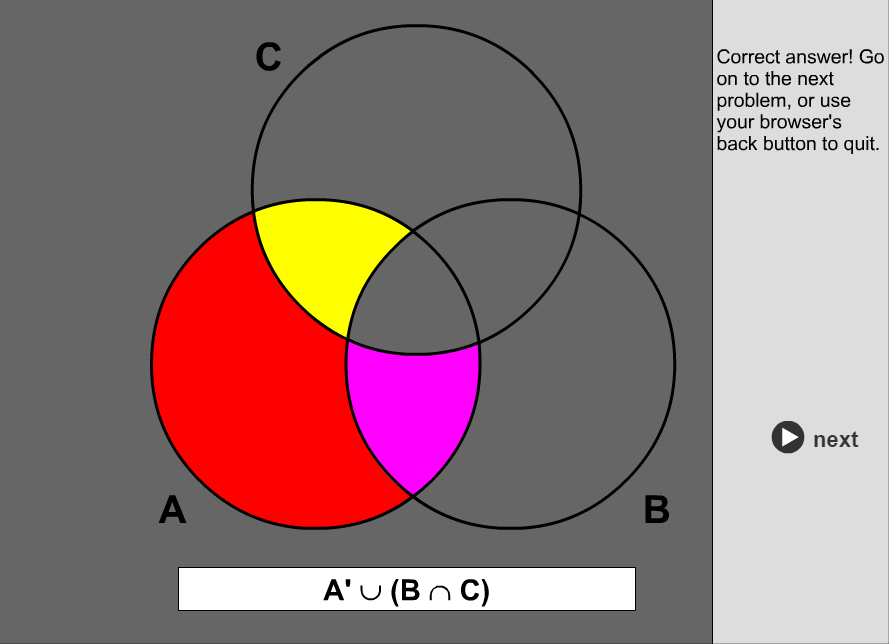
\includegraphics[width=1.0\textwidth]{SOL_set_1_5.png}
			\caption*{$A \prime \cup (B \cap C)$}
			\label{fig:prob_1_5}
		\end{minipage}
		\begin{minipage}{0.5\textwidth}
			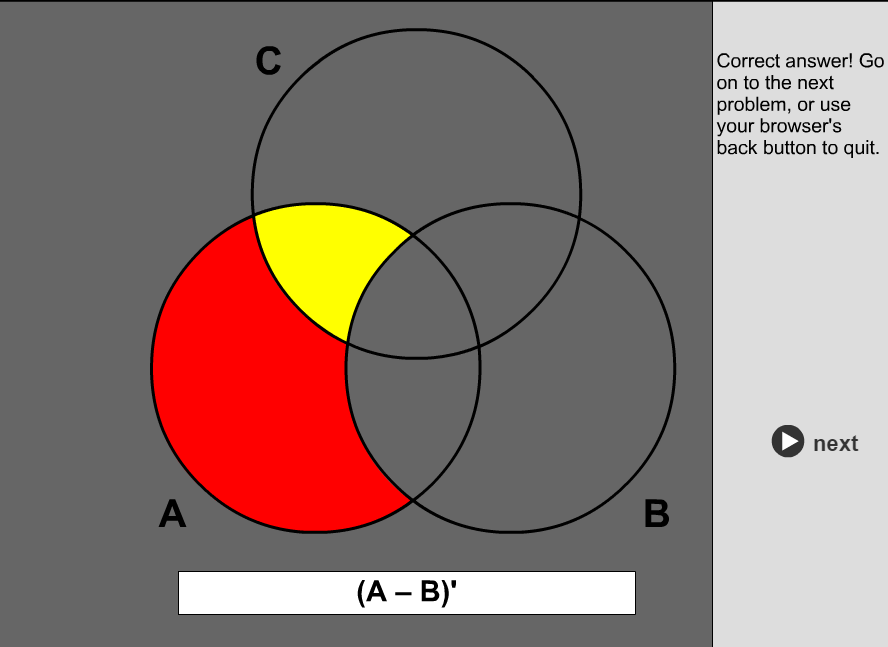
\includegraphics[width=1.0\textwidth]{SOL_set_1_6.png}
			\caption*{$(A-B) \prime$}
			\label{fig:prob_1_6}
		\end{minipage}
	\end{figure}
	\begin{figure}[ht]
		\begin{minipage}{0.5\textwidth}
			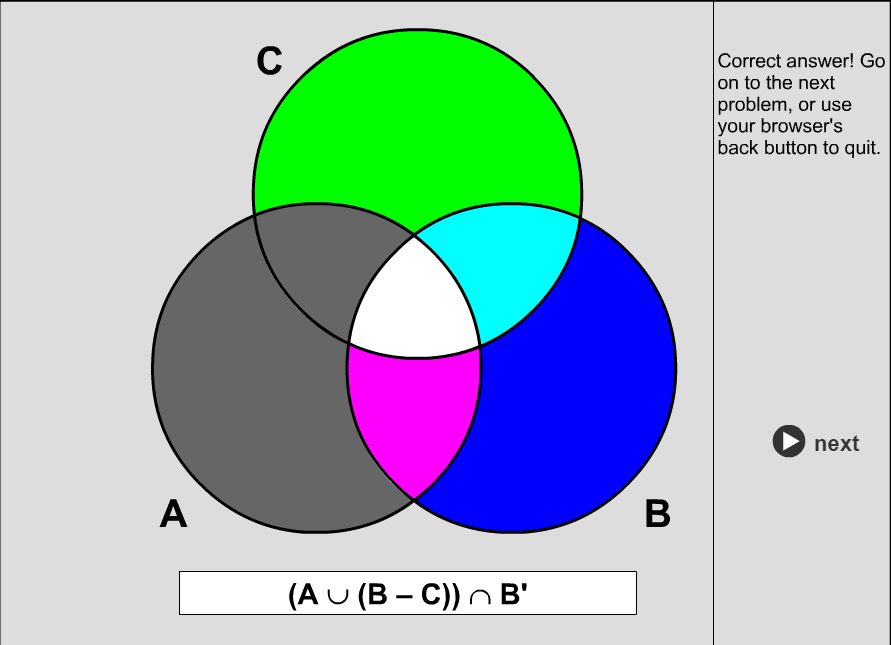
\includegraphics[width=1.0\textwidth]{SOL_set_1_7.png}
			\caption*{$(A \cup (B-C))\cap B \prime $}
			\label{fig:prob_1_7}
		\end{minipage}
	\end{figure}
\newpage
\pdfbookmark[0]{Problem 2}{prob2}
	\section*{Problem 2:}
	Let $A = \{a,b,c\}$, $B=\{x,y\}$, and $C=\{0,1\}$. Find
	\begin{enumerate}
		\item $A \times B$\\
		$\Rightarrow \{(a,x),(a,y),(b,x),(b,y),(c,x),(c,y)\}$
		\item $B \times A$\\
		$\Rightarrow \{(x,a),(x,b),(x,c),(y,a),(y,b),(y,c)\}$
		\item $A \times B \times C$\\
		$\Rightarrow \{(a,x,0),(a,x,1),(a,y,0),(a,y,1),\\
		(b,x,0),(b,x,1),(b,y,0),(b,y,1),\\
		(c,x,0),(c,x,1),(c,y,0),(c,y,1)\}$
		\item $C \times B \times A$\\
		$\Rightarrow \{(0,x,a),(0,x,b),(0,x,c),\\
		(0,y,a),(0,y,b),(0,y,c),\\
		(1,x,a),(1,x,b),(1,x,c),\\
		(1,y,a),(1,y,b),(1,y,c)\}$
		\item $C \times A \times B$\\
		$\Rightarrow \{(0,a,x),(0,a,y),(0,b,x),(0,b,y),(0,c,x),(0,c,y),\\
		(1,a,x),(1,a,y),(1,b,x),(1,b,y),(1,c,x),(1,c,y)\}$
		\item $B \times B \times B$\\
		$\Rightarrow \{(x,x,x),(x,x,y),(x,y,x),(x,y,y),\\
		(y,x,x),(y,x,y),(y,y,x),(y,y,y)\}$
	\end{enumerate}
\newpage
\pdfbookmark[0]{Problem 3}{prob3}
	\section*{Problem 3:}
	Draw the graph of the following linear functions and determine the properties of a function: (domain of a function, range of a function, function is/is not one-to-one function, coordinates of intersections with the x-axis and with the y-axis, local extreme - local minimum \& local maximum)
	\begin{enumerate}
		\item $y=|-x+1|$\\
		\begin{figure}[h]
			\centering
		\begin{minipage}{0.55\textwidth}
			\centering
			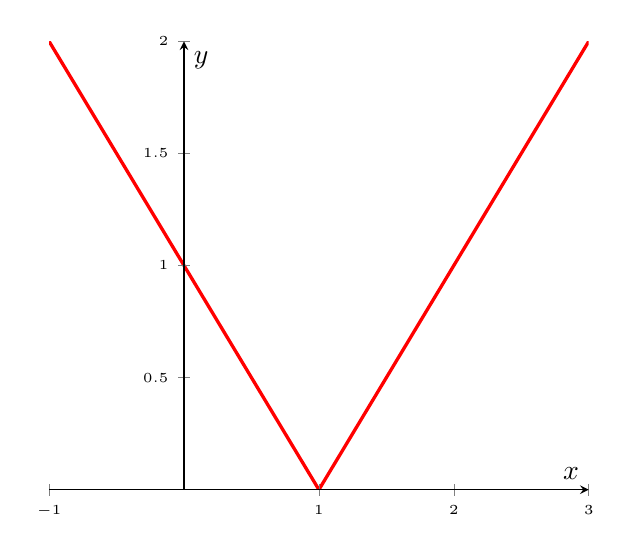
\begin{tikzpicture}
			\begin{axis}[
				axis on top,
				legend pos=outer north east,
				axis lines = center,
				xticklabel style = {font=\tiny},
				yticklabel style = {font=\tiny},
				xlabel = $x$,
				ylabel = $y$,
				legend style={cells={align=left}},
				legend cell align={left},
			]
			\addplot[very thick,red,samples=161,domain=-1:3] {abs(-x+1)};
			\end{axis}
			\end{tikzpicture}
		\end{minipage}
		\begin{minipage}{0.4\textwidth}
			\raggedright
			Domain: $(- \infty,+ \infty)$\\
			Range: $(0,+ \infty)$\\
			Function is not one-to-one\\
			Intersection with the x-axis: $(1,0)$\\
			Intersection with the y-axis: $(0,1)$\\
			Local minimum: $0$
		\end{minipage}
		\end{figure}
		\item $y=-2|4x-8|+3$\\
		\begin{figure}[h]
			\centering
			\begin{minipage}{0.55\textwidth}
				\centering
				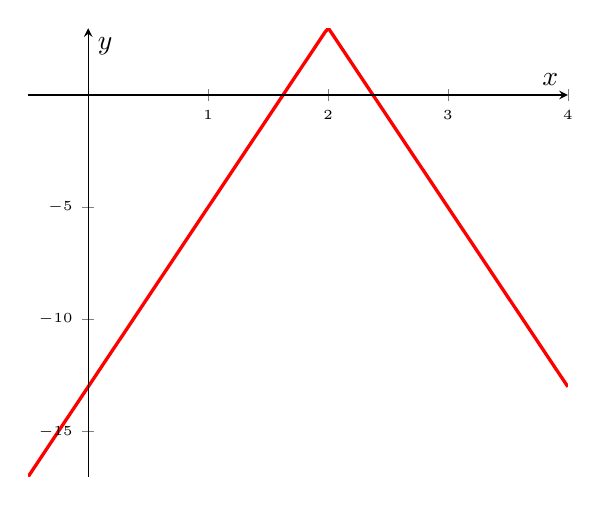
\begin{tikzpicture}
				\begin{axis}[
				axis on top,
				legend pos=outer north east,
				axis lines = center,
				xticklabel style = {font=\tiny},
				yticklabel style = {font=\tiny},
				xlabel = $x$,
				ylabel = $y$,
				legend style={cells={align=left}},
				legend cell align={left},
				]
				\addplot[very thick,red,samples=161,domain=-0.5:4] {-2*abs(4*x-8)+3};
				\end{axis}
				\end{tikzpicture}
			\end{minipage}
			\begin{minipage}{0.4\textwidth}
				\raggedright
				Domain: $(- \infty,+ \infty)$\\
				Range: $(- \infty,3)$\\
				Function is not one-to-one\\
				Intersections with the x-axis: $(\frac{13}{8},0)$ and $(\frac{19}{8},0)$\\
				Intersection with the y-axis: $(0,-14)$\\
				Local maximum: $3$
			\end{minipage}
		\end{figure}
		\item $2x+5y+8=12-4x$
		\begin{figure}[h]
			\centering
			\begin{minipage}{0.55\textwidth}
				\centering
				\begin{tikzpicture}
				\begin{axis}[
				axis on top,
				legend pos=outer north east,
				axis lines = center,
				xticklabel style = {font=\tiny},
				yticklabel style = {font=\tiny},
				xlabel = $x$,
				ylabel = $y$,
				legend style={cells={align=left}},
				legend cell align={left},
				]
				\addplot[very thick,red,samples=161,domain=-1:2] {(4-6*x)/5};
				\end{axis}
				\end{tikzpicture}
			\end{minipage}
			\begin{minipage}{0.4\textwidth}
				\raggedright
				Domain: $(- \infty, + \infty)$\\
				Range: $(- \infty,3)$\\
				Function is one-to-one\\
				Intersection with the x-axis: $(\frac{2}{3},0)$\\
				Intersection with the y-axis: $(0,\frac{4}{5})$\\
				No local extrema
			\end{minipage}
		\end{figure}
	\newpage
		\item $2x+4y-6=0$\\
		\begin{figure}[h]
			\centering
			\begin{minipage}{0.55\textwidth}
				\centering
				\begin{tikzpicture}
				\begin{axis}[
				axis on top,
				legend pos=outer north east,
				axis lines = center,
				xticklabel style = {font=\tiny},
				yticklabel style = {font=\tiny},
				xlabel = $x$,
				ylabel = $y$,
				legend style={cells={align=left}},
				legend cell align={left},
				]
				\addplot[very thick,red,samples=161,domain=-1:4] {(3-x)/2};
				\end{axis}
				\end{tikzpicture}
			\end{minipage}
			\begin{minipage}{0.4\textwidth}
				\raggedright
				Domain: $(- \infty, + \infty)$\\
				Range: $(- \infty,+ \infty)$\\
				Function is one-to-one\\
				Intersection with the x-axis: $(3,0)$\\
				Intersection with the y-axis: $(0,\frac{3}{2})$\\
				No local extrema
			\end{minipage}
		\end{figure}
		\item $y=\frac{2x}{3}-7$\\
		\begin{figure}[h]
			\centering
			\begin{minipage}{0.55\textwidth}
				\centering
				\begin{tikzpicture}
				\begin{axis}[
				axis on top,
				legend pos=outer north east,
				axis lines = center,
				xticklabel style = {font=\tiny},
				yticklabel style = {font=\tiny},
				xlabel = $x$,
				ylabel = $y$,
				legend style={cells={align=left}},
				legend cell align={left},
				]
				\addplot[very thick,red,samples=161,domain=-2:12] {2*x/3 -7};
				\end{axis}
				\end{tikzpicture}
			\end{minipage}
			\begin{minipage}{0.4\textwidth}
				\raggedright
				Domain: $(- \infty, + \infty)$\\
				Range: $(- \infty,+ \infty)$\\
				Function is one-to-one\\
				Intersection with the x-axis: $(\frac{21}{2},0)$\\
				Intersection with the y-axis: $(0,-7)$\\
				No local extrema
			\end{minipage}
		\end{figure}
	\end{enumerate}
\newpage
\pdfbookmark[0]{Problem 4}{prob4}
	\section*{Problem 4:}
	What is the Cartesian product $A \times B$, where $A$ is the set of courses offered by the mathematics department at a university and $B$ is the set of mathematics professors at this university? Give an example of how this Cartesian product can be used.\\
	
	Let:\\
	A = set of courses offered by the mathematics department at a university\\
	B = set of mathematics professors at the university\\
	
	$A \times B = (course, professor|course \in A$ and $professor \in B)$\\
	
	For example, if the university offers algebra and calculus courses and the university has Duo and Marie as math professors:\\
	$A = (algebra, calculus)$\\
	$B = (Duo, Marie)$\\
	$A \times B = \{(algebra, Duo), (algebra, Marie), (calculus, Duo), (calculus, Marie)\}$\\
	
	This Cartesian product can be used to determine all the possible ways for the math professors to teach teach the math courses that the university offers.
\newpage
\pdfbookmark[0]{Problem 5}{prob5}
	\section*{Problem 5:}
	For each of the following functions, find its domain.
	\begin{enumerate}
		\item $f(x) = \frac{\ln (2- \sin (x))}{\sqrt{x^3 -8}}$\\
		$\Rightarrow (2,+\infty)$
		\item $f(x) = \frac{e^x +x^2}{\ln(x-2)}$\\
		$\Rightarrow (0,2) \cup (2,+\infty)$
		\item $f(x) = \ln(|x^2 -4x +3|)$\\
		$\Rightarrow (-\infty, 1) \cup (1,3) \cup (3, +\infty)$
		\item $f(x) = \arcsin(2x -\sqrt{x})$\\
		$\Rightarrow [0,1]$
		\item $f(x) = [\cos(\frac{2}{x})]^x$\\
		$\Rightarrow (-\infty,+\infty)$
	\end{enumerate}
\newpage
\pdfbookmark[0]{Problem 6}{prob6}
	\section*{Problem 6:}
	Prove the following statements
	\begin{enumerate}
		\item $\overline{A \cap B \cap C} = \overline{A} \cup \overline{B} \cup \overline{C}$ (by two ways)\\
		
		\begin{tabular}{r l}
			$\overline{A \cap B \cap C}$ & $= \overline{A} \cup \overline{B} \cup \overline{C}$ (De Morgan's law)
		\end{tabular}
		
		\begin{tabular}{r l}
			$\overline{A \cap B \cap C}$ & $=\{x|x\notin A \cap B \cap C\}$\\
			{} & $=\{x|\neg (x \in A \cap B)\}$\\
			{} & $=\{x|\neg (x\in A \wedge x\in B \wedge x\in C)\}$\\
			{} & $=\{x|\neg(x\in A)\vee\neg(x\in B) \vee\neg(x\in C)\}$\\
			{} & $=\{x|x\notin A \vee x\notin B \vee x\notin C\}$\\
			{} & $=\{x|x\in\overline{A}\vee x\in\overline{B}\vee x\in\overline{C}\}$\\
			{} & $=\{x|x\in\overline{A}\cup\overline{B}\cup\overline{C}\}$
		\end{tabular} 
		\item $P(A) \subseteq P(B)$ if and only if $A \subseteq B$\\
		
		Assume $A \subseteq B$\\
		
		If $P(A)$ contains only the empty set $\emptyset$, then the proof is trivial as any power set contains the empty set $\emptyset$.\\
		If $P(A)$ does not contain only the empty set $\emptyset$, then there exists a set $\{x\}$ in $P(A)$.\\
		
		Let $\{x\}$ be an element of $P(A)$: $x\in P(A)$\\
		Since $A \subseteq B$ and $x \in A$, $x\in B$.\\
		Therefore $\{x\} \in P(B)$.\\
		Hence, every element $x$ in $P(A)$ also has to be in $P(B)$. By the definition of a subset, we conclude that $P(A)$ is a subset of $P(B)$: $P(A) \subseteq P(B)$
		\newpage
		\item $(B-A)\cup(C-A) = (B \cup C)-A$\\
		\begin{figure}[h]
			\centering
			\begin{minipage}{0.5\textwidth}
				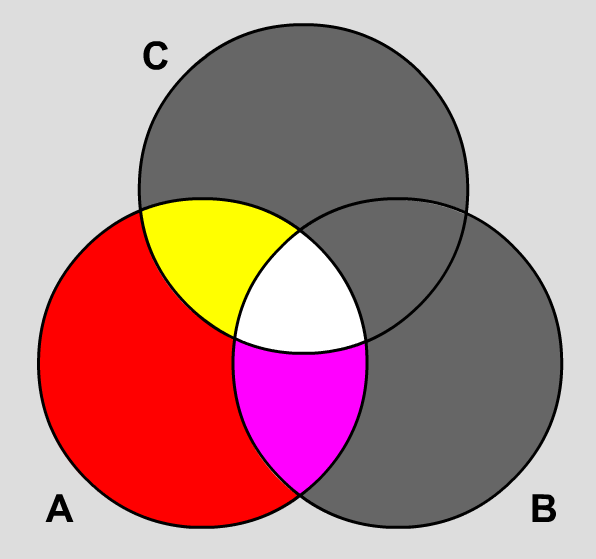
\includegraphics[width=1.0\textwidth]{SOL_set_6_1.png}
				\label{fig:prob_6_1}
			\end{minipage}
		\end{figure}
		\item Explain why $A \times B \times C$ and $(A \times B) \times C$ are not the same\\
		
		Suppose an element of $A$, $B$ and $C$ is $a$, $b$ and $c$ respectively.\\
		$A\times B\times C = (a,b,c)$\\
		$(A\times B)\times C = ((a,b),c)$\\
		
		Therefore $A\times B\times C$ and $(A\times B)\times C$ are not the same.
	\end{enumerate}
\newpage
\pdfbookmark[0]{Problem 7}{prob7}
	\section*{Problem 7:}
	The symmetric difference of $A$ and $B$, denoted by $A \oplus B$, is the set containing those elements in either $A$ or $B$, but not in both $A$ and $B$.
	\begin{enumerate}
		\item Show that $A \oplus B=(A \cup B)(\overline{A \cap B})$\\
		
		\begin{tabular}{r l}
			$A\oplus B$ & $=A\overline{B}+\overline{A}B$\\
			{} & $=A\overline{B}+\overline{A}B+A\overline{A}+\overline{B}B$\\
			{} & $=(A+B)(\overline{A}+\overline{B})$\\
			{} & $=(A+B)(\overline{AB})$\\
			{} & $=(A\cup B)(\overline{A\cap B})$
		\end{tabular}
		\item What can you say about the sets $A$ and $B$ if $A \oplus B=A$?\\
		$\Rightarrow B=\emptyset$
		\item If $A$,$B$, and $C$ are sets, does it follow that $A \oplus (B \oplus C)=(A \oplus B)\oplus C$?\\
		\begin{tabular}{r l}
			$A\oplus(B\oplus C)$ & $=A\oplus (B\overline{C}+\overline{B}C)$\\
			{} & $=A\overline{(B+C)\overline{BC}}+\overline{A}(B\overline{C}+\overline{B}C)$\\
			{} & $=A(\overline{B}\overline{C}+BC)+\overline{A}B\overline{C}+\overline{A}\overline{B}C$\\
			{} & $=A\overline{B}\overline{C}+ABC+\overline{A}B\overline{C}+\overline{A}\overline{B}C$\\
			{} & {}\\
			$(A\oplus B)\oplus C$ & $=(A\overline{B}+\overline{A}B)\oplus C$\\
			{} & $=(A\overline{B}+\overline{A}B)\overline{C}+\overline{(A+B)\overline{AB}}C$\\
			{} & $=A\overline{B}\overline{C}+\overline{A}B\overline{C}+(\overline{A}\overline{B}+AB)C$\\
			{} & $=A\overline{B}\overline{C}+\overline{A}B\overline{C}+\overline{A}\overline{B}C+ABC$
		\end{tabular}\\
		Therefore $A \oplus (B \oplus C)=(A \oplus B)\oplus C$.
	\end{enumerate}
\newpage
\pdfbookmark[0]{Problem 8}{prob8}
	\section*{Problem 8:}
	What can you say about the sets $A$ and $B$ if we know that
	\begin{enumerate}
		\item $A \cup B=A$?\\
		$\Rightarrow B \subset A$
		\item $A \cap B=A$?\\
		$\Rightarrow A \subset B$
		\item $A-B=A$?\\
		$\Rightarrow A \cap B = \emptyset$
		\item $A \cap B=B \cap A$?\\
		True
		\item $A-B=B-A$?\\
		$\Rightarrow A = B$
	\end{enumerate}
\newpage
\pdfbookmark[0]{Problem 9}{prob9}
	\section*{Problem 9:}
	Find the domain and range of these functions. Note that in each case, to find the domain, determine the set of elements assigned values by the function.
	\begin{enumerate}
		\item The function that assigns to each bit string the number of ones in the string minus the number of zeros in the string.\\
		
		Domain = $\{0,1,00,01,11,10,000,001,...\}$\\
		Range = $\mathbb{Z}$
		\item The function that assigns to each bit string twice the number of zeros in that string.\\
		
		Domain = $\{0,1,00,01,11,10,001,...\}$\\
		Range = $\{x|k\in N-\{0\} \rightarrow x=2k\}$
		\item The function that assigns the number of bits left over when a bit string is split into bytes (which are blocks of 8 bits).\\
		
		Domain = $\{0,1,00,01,11,10,001,...\}$\\
		Range = $\{0,1,2,3,4,5,6,7\}$
		\item The function that assigns to each positive integer the largest perfect square not exceeding this integer.\\
		
		Domain = $\mathbb{N}$\\
		Range = $\mathbb{N}$
	\end{enumerate}
\newpage
\pdfbookmark[0]{Problem 10}{prob10}
	\section*{Problem 10:}
	Determine whether each of these functions is a bijection of $\mathbb{R}$ to $\mathbb{R}$.
	\begin{enumerate}
		\item $f(x) = -3x+4$\\
		$y=-3x+4 \Rightarrow x=\frac{4-y}{3}$\\
		Hence the function is a bijection.
		\item $f(x) = -3x^2 +7$\\
		$y=-3x^2 +7 \Rightarrow x^2=\frac{7-y}{3}$\\
		The function is not a bijection.
		\item $f(x) = (x+1)/(x+2)$\\
		There is no real number such that $\frac{x+1}{x+2} =1$, so the function is not a bijection.
		\item $f(x) = x^5 +1$\\
		$y=x^5 +1 \Rightarrow x^5 =y-1$\\
		Therefore the function is a bijection.
		\item $f(x) = \frac{x^2 +1}{x^2 +2}$\\
		There is no real number such that $\frac{x^2+1}{x^2+2}=1$, so the function is not a bijection.
	\end{enumerate}
\newpage
\pdfbookmark[0]{Problem 11}{prob11}
	\section*{Problem 11:}
	If $f$ and $f \circ g$ are one-to-one, does it follow that $g$ is one-to-one? Justify your answer.\\
	Assume:
	\begin{center}
		$g(a)=g(b)$
	\end{center}
	Take function $f$ on both sides:
	\begin{center}
		$f \circ g(a)=f\circ g(b)$
	\end{center}
	Since $f$ is one-to-one:
	\begin{center}
		$a=b$
	\end{center}
	Therefore, $g$ is one-to-one.
\newpage
\pdfbookmark[0]{Problem 12}{prob12}
	\section*{Problem 12:}
	Show that if $x$ is a real number, then $\lceil x \rceil - \lfloor x \rfloor = 1$ if $x$ is not an integer and $\lceil x \rceil - \lfloor x \rfloor = 0$ if $x$ is an integer.\\\\
	For any non-integer real number $x$ exists an integer $n$ such that:
	\begin{center}
		$\lfloor x\rfloor = n$
	\end{center}
	Therefore:
	\begin{center}
		$\lceil x\rceil = n+1$
	\end{center}
	Thus $\lceil x\rceil - \lfloor x\rfloor=1$\\\\
	If $x$ is an integer:
	\begin{center}
		$\lceil x\rceil = x$\\
		$\lfloor x\rfloor = x$
	\end{center}
	Thus $\lceil x\rceil - \lfloor x\rfloor=0$
\newpage
\pdfbookmark[0]{Problem 13}{prob13}
	\section*{Problem 13:}
	For each of these partial functions, determine its domain, codomain, domain of definition, and the set of values for which it is undefined. Also, determine whether it is a total function.
	\begin{enumerate}
		\item $f : \mathbb{Z} \rightarrow \mathbb{R}, f(n)=1/n$\\
		Domain: $\mathbb{Z}$\\
		Codomain: $\mathbb{R}$\\
		Domain of definition: $\mathbb{Z}-\{0\}$
		
		The domain and domain of definition are not the same, so the function is not a total function.
		\item $f:\mathbb{Z} \rightarrow \mathbb{Z},f(n)=\lceil n/2 \rceil$\\
		Domain: $\mathbb{Z}$\\
		Codomain: $\mathbb{Z}$\\
		Domain of definition: $\mathbb{Z}$
		
		The domain and domain of definition are the same, so the function is a total function.
		\item $f:\mathbb{Z} \times \mathbb{Z} \rightarrow \mathbb{Q}, f(m,n)=m/n$\\
		Domain: $\mathbb{Z}\times\mathbb{Z}$\\
		Codomain: $\mathbb{Q}$\\
		Domain of definition: $\mathbb{Z}\times(\mathbb{Z}-\{0\})$
		
		The domain and domain of definition are not the same, so the function is not a total function.
		\item $f:\mathbb{Z} \times \mathbb{Z} \rightarrow \mathbb{Q}, f(m,n)=mn$\\
		Domain: $\mathbb{Z}\times\mathbb{Z}$\\
		Codomain: $\mathbb{Q}$\\
		Domain of definition: $\mathbb{Z}\times\mathbb{Z}$
		
		The domain and domain of definition are the same, so the function is a total function.
		\item $f:\mathbb{Z} \times \mathbb{Z} \rightarrow \mathbb{Q}, f(m,n)=m-n$ if $m>n$\\
		Domain: $\mathbb{Z}\times\mathbb{Z}$\\
		Codomain: $\mathbb{Q}$\\
		Domain of definition: $(m,n)\in\mathbb{Z}\times\mathbb{Z}|m>n$
		
		The domain and domain of definition are not the same, so the function is not a total function.
	\end{enumerate}
\newpage
\pdfbookmark[0]{Problem 14}{prob14}
	\section*{Problem 14:}
	For each of these lists of integers, provide a simple formula or rule that generates the terms of an integer sequence that begins with the given list. Assuming that your formula or rule is correct, determine the next three terms of the sequence.
	\begin{enumerate}
		\item 7, 11, 15, 19, 23, 27, 31, 35, 39, 43, . . .
		\begin{center}
			$a_{n}=a_{n-1} +4$
		\end{center}
		If $a_1 =7$ then:
		\begin{center}
			$a_{11} = 43+4=47$\\
			$a_{12} = 47+4=51$\\
			$a_{13} = 51+4=55$
		\end{center}
		\item 1, 10, 11, 100, 101, 110, 111, 1000, 1001, 1010, 1011, . . .\\
		The sequence is positive integers in increasing order in binary form.\\
		Thus, the next three terms are $1100$, $1101$, $1110$.
		\item 0, 2, 8, 26, 80, 242, 728, 2186, 6560, 19682, . . .
		\begin{center}
			$a_n =3^{n-1}-1$
		\end{center}
		The next three terms are:
		\begin{center}
			$a_{11}=3^{11-1}-1=59048$\\
			$a_{12}=3^{12-1}-1=177146$\\
			$a_{13}=3^{13-1}-1=531440$
		\end{center}
		\item 1, 3, 15, 105, 945, 10395, 135135, 2027025, 34459425, . . .
		\begin{center}
			$a_n=a_{n-1}\cdot(2\cdot n-1)$
		\end{center}
		The next three terms are:
		\begin{center}
			$a_{11}=34459425\cdot(2\cdot11 -1)=654729075$\\
			$a_{12}=654729075\cdot(2\cdot12 -1)=15058768725$\\
			$a_{13}=15058768725\cdot(2\cdot 13-1)=376469218125$
		\end{center}
		\item 1, 0, 0, 1, 1, 1, 0, 0, 0, 0, 1, 1, 1, 1, 1, . . .\\
		The sequence alternates $1$'s and $0$'s and the number of repetition of each term increases repeatedly.\\
		Thus, the next three terms are $0$, $0$, $0$.
	\end{enumerate}
\newpage
\pdfbookmark[0]{Problem 15}{prob15}
	\section*{Problem 15:}
	Find the solution to each of these recurrence relations with the given initial conditions (Hint: Use an iterative approach).
	\begin{enumerate}
		\item $a_n = a_{n-1}, a_0 = 5$
		\begin{center}
			$a_n=5$
		\end{center}
		\item $a_n = a_{n-1} -n,a_0 =4$\\
		\begin{tabular}{l l l}
			$a_n$ & $=a_{n-1}-n$ & {}\\
			{} & $=a_{n-2}-(n-1)-n$ & $=a_{n-2}-2\cdot n+1$\\
			{} & $=a_{n-3}-(n-2)-2\cdot n+1$ & $=a_{n-3}-3\cdot n+1+2$\\
			{} & $=a_{n-4}-(n-3)-3\cdot n+1+2$ & $=a_{n-3}-4\cdot n+1+2+3$\\
			\multicolumn{3}{c}{...}\\
			{} & $=a_{n-n}-n\cdot n+\sum_{i=0}^{n-1}i$ & {}\\
			{} & $=a_0-n^2+\frac{n(n+1)}{2}$ & $=a_0+\frac{1}{2}n-\frac{1}{2}n^2$\\
			{} & $=4+\frac{1}{2}n-\frac{1}{2}n^2$ & {}
		\end{tabular}
		\item $a_n = 2a_{n-1} -3, a_0 =-1$\\
		\begin{tabular}{l l l}
			$a_n$ & $=2a_{n-1}-3$ & {}\\
			{} & $=2(2a_{n-2}-3)-3$ & $=2^2a_{n-2}-3(1+2)$\\
			{} & $=2^2(2a_{n-3}-3)-3(1+2)$ & $=2^3a_{n-3}-3(1+2+2^2)$\\
			{} & $=2^3(2a_{n-4}-3)-3(1+2+2^2)$ & $=2^4a_{n-2}-3(1+2+2^2+2^3)$\\
			\multicolumn{3}{c}{...}\\
			{} & $=2^na_{n-n}-3\sum_{i=0}^{n-1}2^i$ & {}\\
			{} & $=2^na_0-3\sum_{i=0}^{n-1}2^i$ & $=-2^n-3\frac{2^n-1}{2-1}$\\
			{} & $=-2^n-3\cdot2^n+3$ & $=-4\cdot2^n+3$\\
		\end{tabular}
		\item $a_n = (n+1)a_{n-1}, a_0 =2$\\
		\begin{tabular}{l l l}
			$a_n$ & $=(n+1)a_{n-1}$ & {}\\
			{} & $=(n+1)na_{n-2}$ & $=(n+1)n(n-1)a_{n-3}$\\
			\multicolumn{3}{c}{...}\\
			{} & $=(n+1)!a_{n-n}$ & $=(n+1)!a_0$\\
			{} & $=2(n+1)!$ & {}
		\end{tabular}
	\newpage
		\item $a_n = -a_{n-1}+n-1, a_0 =7$\\
		\begin{tabular}{l l}
			$a_n$ & $=-a_{n-1}+n-1$\\
			{} & $=-(-a_{n-2}+n-1-1)+n-1$\\ {} & $=(-1)^2 a_{n-2}+(n-1)-(n-2)$\\
			{} & $=(-1)^2(-a_{n-3}+n-2-1)+(n-1)-(n-2)$\\ {} & $=(-1)^3a_{n-3}+(n-1)-(n-2)+(n-3)$\\
			\multicolumn{2}{c}{...}\\
			{} & $=(-1)^na_{n-n}+\sum_{i=0}^{n-1}(-1)^{n-i+1}i$\\
			{} & $=(-1)^na_0+\sum_{i=0}^{n-1}(-1)^{n-i+1}i$\\
			{} & $=(-1)^n\cdot7+\sum_{i=0}^{n-1}(-1)^{n-i+1}i$
		\end{tabular}
	\end{enumerate}
\newpage
\pdfbookmark[0]{Rosen's Book}{rosen}
	\section*{Rosen's book}
\pdfbookmark[1]{2.1}{2.1}
	\subsection*{2.1:}
\pdfbookmark[2]{9}{2.1.9}
	\subsubsection*{9:}
	Determine whether each of these statements is true or false.
	\begin{enumerate}[label=\textbf{$\alph*$)}]
		\item $0\in\emptyset$\\
		$\Rightarrow$ False
		\item $\emptyset\in\{0\}$\\
		$\Rightarrow$ False
		\item $\{0\}\subset\emptyset$\\
		$\Rightarrow$ False
		\item $\emptyset\subset\{0\}$\\
		$\Rightarrow$ True
		\item $\{0\}\in\{0\}$\\
		$\Rightarrow$ False
		\item $\{0\}\subset\{0\}$\\
		$\Rightarrow$ True
		\item $\{\emptyset\}\subseteq\{\emptyset\}$\\
		$\Rightarrow$ True
	\end{enumerate}
\pdfbookmark[2]{10}{2.1.10}
	\subsubsection*{10:}
	Determine whether these statements are true or false.
	\begin{enumerate}[label=\textbf{$\alph*$)}]
		\item $\emptyset\in\{\emptyset\}$\\
		$\Rightarrow$ True
		\item $\emptyset\in\{\emptyset,\{\emptyset\}\}$\\
		$\Rightarrow$ True
		\item $\{\emptyset\}\in\{\emptyset\}$\\
		$\Rightarrow$ False
		\item $\{\emptyset\}\in\{\{\emptyset\}\}$\\
		$\Rightarrow$ True
		\item $\{\emptyset\}\subset\{\emptyset,\{\emptyset\}\}$\\
		$\Rightarrow$ True
		\item $\{\{\emptyset\}\}\subset\{\emptyset,\{\emptyset\}\}$\\
		$\Rightarrow$ True
		\item $\{\{\emptyset\}\}\subset\{\{\emptyset\},\{\emptyset\}\}$\\
		$\Rightarrow$ False
		\end{enumerate}
\pdfbookmark[2]{22}{2.1.22}
	\subsubsection*{22:}
	Can you conclude that $A=B$ if $A$ and $B$ are two sets with the same power set?\\
	
	By definition, $\wp(A)$ is the set of all subsets that can be generated from $A$, thus $A$ is the largest set in $\wp(A)$.
	
	Therefore, if $\wp(A)=\wp(B)$ then $A=B$.
\pdfbookmark[2]{26}{2.1.26}
	\subsubsection*{26}
	Show that if $A\subseteq C$ and $B\subseteq D$, then $A\times B\subseteq C\times D$\\
	
	Suppose $x$, $y$ are elements of $A$ and $B$ respectively.\\
	By the definition of the Cartesian product:
	\begin{center}
		$(x,y)\in A\times B$
	\end{center}
	Since $A\subseteq C$ and $B\subseteq D$, we can conclude $x\in C$ and $y\in D$.\\
	By the definition of the Cartesian product:
	\begin{center}
		$(x,y)\in C\times D$
	\end{center}
	Therefore, every element $(x,y)$ in $A\times B$ has to be in $C\times D$, hence $A\times B$ is a subset of $C\times D$.
	\begin{center}
		$A\times B\subset C\times D$
	\end{center}
\pdfbookmark[2]{29}{2.1.29}
	\subsubsection*{29:}
	What is the Cartesian product $A\times B\times C$, where $A$ is the set of all airlines and $B$ and $C$ are both the set of all cities in the United States? Give an example of how this Cartesian product can be used.\\\\
	$A\times B\times C=\{(airline,city1,city2)|airline\in A\vee city1\in B\vee city2\in C\}$\\\\
	For example:
	
	$A=\{Vietnam\; Airlines, Qatar\}$
	
	$B=\{New\; York, Washington\}$
	
	$C=\{Kansas, Chicago\}$\\
	\begin{tabular}{l l}
		$A\times B\times C=$ & $\{(Vietnam\;Airlines,New\;York,Kansas),$\\
		{} & $ (Vietnam\;Airlines,New\;York,Chicago),$\\
		{} & $(Vietnam\;Airlines,Washington,Kansas),$\\
		{} & $(Vietnam\;Airlines, Washington, Chicago),$\\
		{} & $(Qatar,New\;York,Kansas),$\\
		{} & $(Qatar,New\;York,Chicago),$\\
		{} & $(Qatar,Washington,Kansas),$\\
		{} & $(Qatar, Washington, Chicago)\}$
	\end{tabular}\\
	This Cartesian product can be used to determine all possible flights airlines can offer between two cities.
\pdfbookmark[2]{40}{2.1.40}
	\subsubsection*{40:}
	Explain why $(A\times B)\times(C\times D)$ and $A\times (B\times C)\times D$ are not the same.
	
	Suppose:
	\begin{center}
		$a\in A$\\
		$b\in B$\\
		$c\in C$\\
		$d\in D$
	\end{center}

	$(A\times B)\times(C\times D)$\\
	$=\{((a,b),(c,d))\}$
	
	$A\times(B\times C)\times D$\\
	$=\{(a,(b,c),d)\}$\\\\
	Hence, they are not the same.
\newpage
\pdfbookmark[1]{2.2}{2.2}
	\subsection*{2.2:}
\pdfbookmark[2]{2}{2.2.2}
	\subsubsection*{2:}
	Suppose that $A$ is the set of sophomores at your school and $B$ is the set of students in discrete mathematics at your school. Express each of these sets in terms of $A$ and $B$.
	\begin{enumerate}[label=\textbf{\alph*)}]
		\item the set of sophomores taking discrete mathematics in your school\\
		$\Rightarrow A\cap B$
		\item the set of sophomores at your school who are not taking discrete mathematics\\
		$\Rightarrow A-B$
		\item the set of students at your school who either are sophomores or are taking discrete mathematics\\
		$\Rightarrow A\cup B$
		\item the set of students at your school who either are not sophomores or are not taking discrete mathematics\\
		$\Rightarrow \overline{A}\cup \overline{B}$
	\end{enumerate}
\pdfbookmark[2]{30}{2.2.30}
	\subsubsection*{30:}
	Can you conclude that $A=B$ if $A$,$B$, and $C$ are sets such that
	\begin{enumerate}[label=\textbf{\alph*)}]
		\item $A\cup C=B\cup C$?\\
		$\Rightarrow$ No
		\item $A\cap C=B\cap C$?\\
		$\Rightarrow$ No
		\item $A\cup C=B\cup C$ and $A\cap C=B\cap C$?\\
		$\Rightarrow$ Yes
	\end{enumerate}
\begin{comment}
\pdfbookmark[2]{41}{2.2.41}
	\subsubsection*{41:}
	Suppose that $A$, $B$, and $C$ are sets such that $A\oplus C=B\oplus C$. Must it be the case that $A=B$?
	
	$A\oplus C=B\oplus C$\\
	$\Leftrightarrow A\cup C-A\cap C=B\cup B-B\cap C$\\
	Suppose that $x\in A$.
	
	Case $x\in C$\\
	Then $x\in A\cap C$ which implies that $x\notin A\oplus C$, thus $x\notin B\oplus C$ and $x\in B$.
	
	Case $x\notin C$\\
	Then $x\in A\oplus C$ which implies that $x\in B\oplus C$ or $x\notin B$.\\\\
	In conclusion, if $x\in A$ then $x\in B$, or $A=B$.
\pdfbookmark[2]{46}{2.2.46}
	\subsubsection*{46:}
	Show that if $A$, $B$, and $C$ are sets, then
	
	$|A\cup B\cup C|=|A|+|B|+|C|-|A\cap B|-|A\cap C|-|B\cap C|+|A\cap B\cap C|$\\\\
	Because every element in $A\cup B\cup C$ is in one of the sets in $A$, $B$ or $C$:
	\begin{center}
	$|A\cup B\cup C| \leq |A|+|B|+|C|$
	\end{center}
	For every element in $A\cap B$, we have counted it twice. The same problem applies for $B\cap C$ and $A\cap C$. Therefore we need to subtract the cardinality of these sets. The cardinality of $A\cap B\cap C$ is not affected.
	\begin{center}
		$|A\cup B\cup C| = |A|+|B|+|C|-|A\cap B|-|A\cap C|-|B\cap C|+|A+B+C|$
	\end{center}
\end{comment}
\pdfbookmark[2]{61}{2.2.61}
	\subsubsection*{61:}
	Let $A$ and $B$ be the multisets $\{3\cdot a,2\cdot b,1\cdot c\}$ and $\{2\cdot a,3\cdot b,4\cdot d\}$, respectively. Find
	\begin{enumerate}[label=\textbf{\alph*)}]
		\item $A\cup B$\\
		$=\{3\cdot a,3\cdot b,1\cdot c,4\cdot d\}$
		\item $A\cap B$\\
		$=\{2\cdot a,2\cdot b\}$
		\item $A-B$\\
		$=\{1\cdot a,1\cdot c\}$
		\item $B-A$\\
		$=\{1\cdot b,4\cdot d\}$
		\item $A+B$\\
		$=\{5\cdot a,5\cdot b,1\cdot c,4\cdot d\}$
	\end{enumerate}
\pdfbookmark[2]{62}{2.2.62}
	\subsubsection*{62:}
	Suppose that $A$ is the multiset that has as its elements the types of computer equipment needed by one department of a university and the multiplicities are the number of pieces of each type needed, and $B$ is the analogous multiset for a second department of the university. For instance, $A$ could be the multiset $\{107\cdot personal\;computers,44\cdot routers,6\cdot servers\}$ and $B$ could be the multiset $\{14\cdot personal\;computers, 6\cdot routers,2\cdot mainframes\}$.
	\begin{enumerate}[label=\textbf{\alph*)}]
		\item What combination of $A$ and $B$ represents the equipment the university should buy assuming both departments use the same equipment?
		
		$A\cup B=\{107\cdot personal\;computers,44\cdot routers,6\cdot servers,2\cdot mainframes\}$
		\item What combination of $A$ and $B$ represents the equipment that will be used by both departments if both departments use the same equipment?
		
		$A\cap B=\{14\cdot personal\;computers,6\cdot routers\}$
		\item What combination of $A$ and $B$ represents the equipment that the second department uses, but the first department does not, if both departments use the same equipment?
		
		$B-A=\{2\cdot mainframes\}$
		\item What combination of $A$ and $B$ represents the equipment that the university should purchase if the departments do not share equipment?
		
		$A+B=\{121\cdot personal\;computers,50\cdot routers,6\cdot servers,2\cdot mainframes\}$
	\end{enumerate}
\newpage
\pdfbookmark[1]{2.3}{2.3}
	\subsection*{2.3:}
\pdfbookmark[2]{6}{2.3.6}
	\subsubsection*{6:}
	Find the domain and range of these functions.
	\begin{enumerate}[label=\textbf{\alph*)}]
		\item the function that assigns to each pair of positive integers the first integer of the pair\\\\
		Domain: $(\mathbb{N}-\{0\})\times(\mathbb{N}-\{0\})$\\
		Range: $\mathbb{N}-\{0\}$
		\item the function that assigns to each positive integer its largest decimal digit\\\\
		Domain: $\mathbb{N}-\{0\}$\\
		Range: $\{1,2,3,4,5,6,7,8,9\}$
		\item the function that assigns to a bit string the number of ones minus the number of zeros in the string\\\\
		Domain: $\{0,1,00,01,10,11,000,001,...\}$\\
		Range: $\mathbb{Z}$
		\item the function that assigns to each positive integer the largest integer not exceeding the square root of the integer\\\\
		Domain: $\mathbb{N}-\{0\}$\\
		Range: $\mathbb{N}-\{0\}$
		\item the function that assigns to a bit string the longest string of ones in the string\\\\
		Domain: $\{0,1,00,01,10,11,000,001,...\}$\\
		Range: $\{1,11,111,1111,...\}$
	\end{enumerate}
\pdfbookmark[2]{15}{2.3.15}
	\subsubsection*{15:}
	Determine whether the function $f:\mathbb{Z}\times\mathbb{Z}\rightarrow\mathbb{Z}$ is onto if
	\begin{enumerate}[label=\textbf{\alph*)}]
		\item $f(m,n)=m+n$.\\
		$\Rightarrow$ Onto
		\item $f(m,n)=m^2+n^2$.\\
		$\Rightarrow$ Not onto
		\item $f(m,n)=m$.\\
		$\Rightarrow$ Onto
		\item $f(m,n)=|n|$.\\
		$\Rightarrow$ Not onto
		\item $f(m,n)=m-n$.\\
		$\Rightarrow$ Onto
	\end{enumerate}
\pdfbookmark[2]{26}{2.3.26}
	\subsubsection*{26:}
	\begin{enumerate}[label=\textbf{\alph*)}]
		\item Prove that a strictly increasing function from $\mathbf{R}$ to itself is one-to-one.
		\begin{center}
			$f:\mathbf{R}\rightarrow\mathbf{R}$
		\end{center}
		$f$ is strictly increasing, if $x<y$ then $f(x)<f(y)$.\\
		Assume:
		\begin{center}
			$f(a)=f(b)$
		\end{center}
		If $a<b$ then $f(a)<f(b)$, thus the assumption is wrong.
		
		If $a>b$ then $f(a)>f(b)$, thus the assumption is wrong.
		
		Therefore:
		\begin{center}
			$a=b$
		\end{center}
		In other words, $f$ is one-to-one.
		\item Give an example of an increasing function from $\mathbf{R}$ to itself that is not one-to-one.\\\\
		$f(x)=\lfloor x\rfloor$ is increasing but not one-to-one.
		\begin{center}
			$f(1)=1$\\
			$f(1.5)=1$
		\end{center}
	\end{enumerate}
\pdfbookmark[2]{35}{2.3.35}
	\subsubsection*{35:}
	If $f$ and $f \circ g$ are onto, does it follow that $g$ is onto? Justify your answer.\\\\
	Suppose $A=\{0\}$, $B=\{0,1\}$, $C=\{0\}$ and
	\begin{center}
		$g(0)=0$\\
		$f(0)=0$\\
		$f(1)=0$
	\end{center}
	$f$ is then onto, because for every element $x\in C$, there exists an element $y\in B$ such that $f(y)=x$.\\
	$f\circ g$ is also onto, because for every element $x\in C$, there exists an element $y\in B$ such that $f\circ g(y)=x$.\\
	However, $1$ is an element of $B$ but $1$ is not the image of any element in $A$, thus $g$ is not onto.
\pdfbookmark[2]{44}{2.3.44}
	\subsubsection*{44:}
	Let $f$ be a function from $A$ to $B$. Let $S$ and $T$ be subsets of $B$. Show that
	\begin{enumerate}[label=\textbf{\alph*)}]
		\item $f^{-1}(S\cup T)=f^{-1}(S)\cup f^{-1}(T)$.\\
		
		We have $f^{-1}(S)=\{x\in A:f(x)\in S\}$ as a premise. Therefore, $x\in f^{-1}(S)$ if and only if $f(x)\in S$.\\
		
		$x\in f^{-1}(S\cup T)$\\
		$\Leftrightarrow f(x)\in S\cup T$\\
		$\Leftrightarrow f(x)\in S\cup f(x)\in T$\\
		$\Leftrightarrow x\in f^{-1}(S)\cup x\in f^{-1}(T)$\\
		$\Rightarrow f^{-1}(S\cup T)=f^{-1}(S)\cup f^{-1}(T)$
		\item $f^{-1}(S\cap T)=f^{-1}(S)\cap f^{-1}(T)$.\\
		
		$x\in f^{-1}(S\cap T)$\\
		$\Leftrightarrow f(x)\in S\cap T$\\
		$\Leftrightarrow f(x)\in S\cap f(x)\in T$\\
		$\Leftrightarrow x\in f^{-1}(S)\cap x\in f^{-1}(T)$\\
		$\Rightarrow f^{-1}(S\cap T)=f^{-1}(S)\cap f^{-1}(T)$
	\end{enumerate}
\pdfbookmark[2]{51}{2.3.51}
	\subsubsection*{51:}
	Show that if $x$ is a real number and $n$ is an integer, then
	\begin{enumerate}[label=\textbf{\alph*)}]
		\item $x<n$ if and only if $\lfloor x\rfloor <n$.\\\\
		We have $x<n$ and $\lfloor x\rfloor<x$, thus $\lfloor x\rfloor<n$.\\\\
		We have $\lfloor x\rfloor<x<\lfloor x+1\rfloor$. Since $n$ is an integer and $\lfloor x\rfloor<n$, $\lfloor x+1\rfloor\leq n$.\\
		Therefore, $x<n$.
		\item $n<x$ if and only if $n<\lceil x\rceil$.\\\\
		We have $n<x$ and $x<\lceil x\rceil$, thus $n<\lceil x\rceil$.\\\\
		We have $\lceil x-1\rceil<x<\lceil x\rceil$. Since $n$ is an integer and $n<\lceil x\rceil$, $n\leq\lceil x-1\rceil$.\\
		Therefore, $n<x$.
	\end{enumerate}
\pdfbookmark[2]{71}{2.3.71}
	\subsubsection*{71:}
	Let $S$ be a subset of a universal set $U$. The \textbf{characteristic function} $f_S$ of $S$ is the function from $U$ to the set $\{0,1\}$ such that $f_S(x)=1$ if $x$ belongs to $S$ and $f_S(x)=0$ if $x$ does not belong to $S$. Let $A$ and $B$ be sets. Show that for all $x\in U$,
	\begin{enumerate}[label=\textbf{\alph*)}]
		\item $f_{A\cap B}(x)=f_A(x)\cdot f_B(x)$\\\\
		Assume $f_{A\cap B}(x)=1$\\
		$\Leftrightarrow x\in A\cap B$\\
		$\Leftrightarrow (x\in A)\cap (x\in B)$\\
		$\Leftrightarrow f_A(x)=1\cap f_B(x)=1$\\
		$\Leftrightarrow f_A(x)\cdot f_B(x)=1$\\
		
		Therefore, $f_{A\cap B}(x)=1$ if and only if $f_A(x)\cdot f_B(x)=1$. Thus, the functions have to be equal.
		\item $f_{A\cup B}(x)=f_A(x)+f_B(x)-f_A(x)\cdot f_B(x)$\\\\
		Assume $f_{A\cup B}(x)=1$\\
		$\Leftrightarrow x\in A\cup B$\\
		$\Leftrightarrow x\in A\cup x\in B$\\
		$\Leftrightarrow f_A(x)=1\cup f_B(x)=1$\\
		$\Leftrightarrow \neg(\neg(f_A(x)=1)\cup(f_B(x)=1))$\\
		$\Leftrightarrow \neg(\neg(f_A(x)=1)\cap\neg(f_B(x)=1))$\\
		$\Leftrightarrow \neg(f_A(x)=0\cap f_B(x)=0)$\\
		
		$f_A(x)+f_B(x)-f_A(x)\cdot f_B(x)=0$ if and only if $f_A(x)=0$ and $f_B(x)=0$. Thus $f_A(x)+f_B(x)-f_A(x)\cdot f_B(x)=1$ if and only if $f_A(x)\neq0$ or $f_B(x)\neq0$.\\
		$\Leftrightarrow f_A(x)+f_B(x)-f_A(x)\cdot f_B(x)=1$\\
		
		Therefore, $f_{A\cup B}(x)=1$ if and only if $f_A(x)+f_B(x)-f_A(x)\cdot f_B(x)=1$. Thus, the functions are equal.
		\item $f_{\overline{A}}(x)=1-f_A(x)$
		\item $f_{A\oplus B}(x)=f_A(x)+f_B(x)-2f_A(x)f_B(x)$
	\end{enumerate}
\newpage
\pdfbookmark[1]{2.4}{2.4}
	\subsection*{2.4:}
\pdfbookmark[2]{13}{2.4.13}
	\subsubsection*{13:}
\pdfbookmark[2]{15}{2.4.15}
	\subsubsection*{13:}
\pdfbookmark[2]{17}{2.4.17}
	\subsubsection*{17:}
\pdfbookmark[2]{19}{2.4.19}
	\subsubsection*{19:}
\pdfbookmark[2]{25}{2.4.25}
	\subsubsection*{25:}
\pdfbookmark[2]{41}{2.4.41}
	\subsubsection*{41:}
\newpage
\pdfbookmark[1]{2.5}{2.5}
	\subsection*{2.5:}
\pdfbookmark[2]{3}{2.5.3}
	\subsubsection*{3:}
\pdfbookmark[2]{19}{2.5.19}
	\subsubsection*{19:}
\newpage
\pdfbookmark[1]{5.1}{5.1}
	\subsection*{5.1:}
\pdfbookmark[2]{13}{5.1.13}
	\subsubsection*{13:}
\pdfbookmark[2]{32}{5.1.32}
	\subsubsection*{32:}
\newpage
\pdfbookmark[1]{8.2}{8.2}
	\subsection*{8.2:}
\pdfbookmark[2]{16}{8.2.16}
	\subsubsection*{16:}
\pdfbookmark[2]{26}{8.2.26}
	\subsubsection*{26:}
\pdfbookmark[2]{30}{8.2.30}
	\subsubsection*{30:}
\end{document}